\documentclass[a4paper,12pt]{report}
\usepackage{fancyhdr}
\usepackage[pdftex]{graphicx}
\usepackage[pdftex,colorlinks,bookmarksopen]{hyperref}
\usepackage{color}
\usepackage{framed}
\usepackage{listings}
\usepackage{enumitem}
\usepackage{tikz}

\begin{document}

\addtolength{\textheight}{2cm}
\addtolength{\topmargin}{-1cm}

\lstnewenvironment{CS}{\lstset{language=[Sharp]C,frame=single,belowskip=0.5cm,breaklines=true,prebreak=\ldots}}{}

\newenvironment{note}
{\vspace*{5mm}\begin{framed}\rule{1ex}{1ex}\hspace{\stretch{1}} Note: }
{\hspace{\stretch{1}}\rule{1ex}{1ex}\end{framed}}

% \newcommand{\kw}{\it}
% \newcommand{\new}{\bf}
% \newcommand{\comment}{\it}

\title{ZBox\\Guide}
\author{Arthur Zaczek}
\author{David Schmitt}

\pagestyle{empty}

\begin{figure}
	
\includegraphics[width=0.4\textwidth]{images/logo.png}
\end{figure}
\hrule

\vspace*{1.5cm}

\begin{center}
 {\huge \bf Kistl Guide }
\end{center}

\vspace*{1cm}

\begin{center}
{\huge The Hitchhiker's guide to the Kistl galaxy }
\end{center}




\tableofcontents

\setlength{\headheight}{15pt}

\pagestyle{fancy}

\renewcommand{\chaptermark}[1]{\markboth{\chaptername\ \thechapter.\ #1}{}}
\renewcommand{\sectionmark}[1]{\markright{\thesection.\ #1}}

\newenvironment{descriptionBorder}
{
  \begin{framed}
  \begin{description}[labelindent=3mm,leftmargin=*,topsep=0mm]
}
{
  \end{description}
  \end{framed}
}

\chapter{Introduction}

Zetbox is a application framework to provide the complete process from
defining data structures, designing data access and transfer objects,
designing servers and GUIs and the necessary parts to make everything
work together.

\section{Zetbox Basic}
Zetbox Basic provides the folowing services:

\begin{descriptionBorder}
\item[Module editor] { All meta informations are defined by the module editor }
\item[Database Provider] { The Database provider manages database access.
Currently SQL Server 2008 \& PosgreSQL are supported. }
\end{descriptionBorder}

\chapter{Programming}
\chapter{Programming}

This chapter describes the various ways and pieces the Kistl system is
programmed and customized.

\section{Objects}

\section{Modules}

\section{Enhancing Kistl's inner workings}

\subsection{Database Providers}

\section{Graphical User Interface}

Like other subsystems, the GUI core is designed to be platform
independent. Therefore only the "outermost" shell contains toolkit
specific code.

\subsection{Architecture}

The GUI is modeled after the Model-View-ViewModel architecture. The
\emph{Model} represents the underlying data structures and business
logic. It is provided by the generated classes from the actual
datamodel. \emph{View Models} provide display specific functionality
like formatting, transient state holding and implementing the user's
possible actions. They always inherit from
\texttt{Kistl.Client.Presentables.PresentableModel}. Common
implementations reside in the \texttt{Kistl.Client.Presentables}
namespace. Finally, \emph{Views} (editors and displays) are the actual
components taking care of showing content to the user and converting the
users keypresses and clicks into calls on the view models interface.
Views are toolkit\footnote{Toolkits are GUI libraries like GTK\# or
Windows Forms.} specific and reside in the toolkit's respective
assembly.



\chapter{Management}
\section{Access Rights}

Managing access to objects has to be fine-grained, flexible, fast and robust.
To achieve these goals, the Kistl combines an expressive set of rules and
generated rights tables.

\subsection{Roles}

To decouple users from the specifics of access management, rights are only
conferred to roles, which in turn are assumed by users through their membership
in groups and relations. 

As an example, consider the project. The project's manager will always have
special access rights on the project, regardless of who actually fills this
role. Formulating access rights relative to such roles makes them more robust
against changes in the people's responsibilities, since when the project manager
changes all his rights automatically follow.

\subsubsection{Groups}

The easiest kind of role is the \emph{Group}. Applicability of this role is only
defined through membership in the group and is independent of any other
relationships.

\subsubsection{Instance-specific roles}

Instance-specific roles are conferred through specified relationships with
business objects. One example already mentioned is the project's \emph{Manager}.
Another the \emph{assigned employees} for a project.

\subsubsection{Transitive roles}

In some cases the role is not directly associated with the business object under
consideration. Instead the connection spans over one or more navigational
properties. An example would be access to the set of \emph{Tasks} contained in a
project, which is granted by virtue of being an assigned employee of the
project.

\subsubsection{Nested roles}

Finally, roles can be members of groups or roles. This allows for the definition
of groups like \emph{all project managers}, which for example might be granted
rights on a special set of documents pertaining to management procedures.

\subsection{Rules}

Rules are the way to specify how rights are assigned to roles. There are global,
\emph{ObjectClass}-specific and instance-specific rules. 

Global rules can be used for granting blanket administrative access or for
privileged transfer or analysis processes.

ObjectClass-specific rules are useful for defining class-specific
administrators, journalling classes (insert only) and other special cases.

Finally, instance-specific rules allow the most flexible and fine-grained access
control, by defining cascading rights through various mechanisms. All such rules
specify the set of roles for which the rule is applicable, the set of instances
which are affected by this rule and the set of granted rights.

\subsubsection{Instance-specific rules}

First, an example: all employees assigned to a project are allowed to edit the
associated tasks of the project. As an instance-specific rule, this would read:
"\emph{Project}: Grant READ,WRITE on \emph{Tasks} to \emph{Employees}."

The set of roles can be specified by a navigator from the current instance to a
single Identity or a set of Identities, by a constant set of groups or as a set
of necessary access rights to the current instance.

The set of affected instances can be specified by a direct navigator from the
current instance, or by using the instance itself.



\chapter{\label{Packaging}Packaging}
This chapter describes the way how modules (packages) are transfered between Kistl installations.

\section{\label{Packaging_Content_of_a_package}Content of a package}

A package contains schema information, meta data, object instances and code. See \ref{content_of_package} for details. 
A package can contain one or more modules. A package is a zip file that contains one or more XML files containing meta information and/or data and binary files like icons or assemblies.

\begin{figure}[ht]
	\begin{center}
		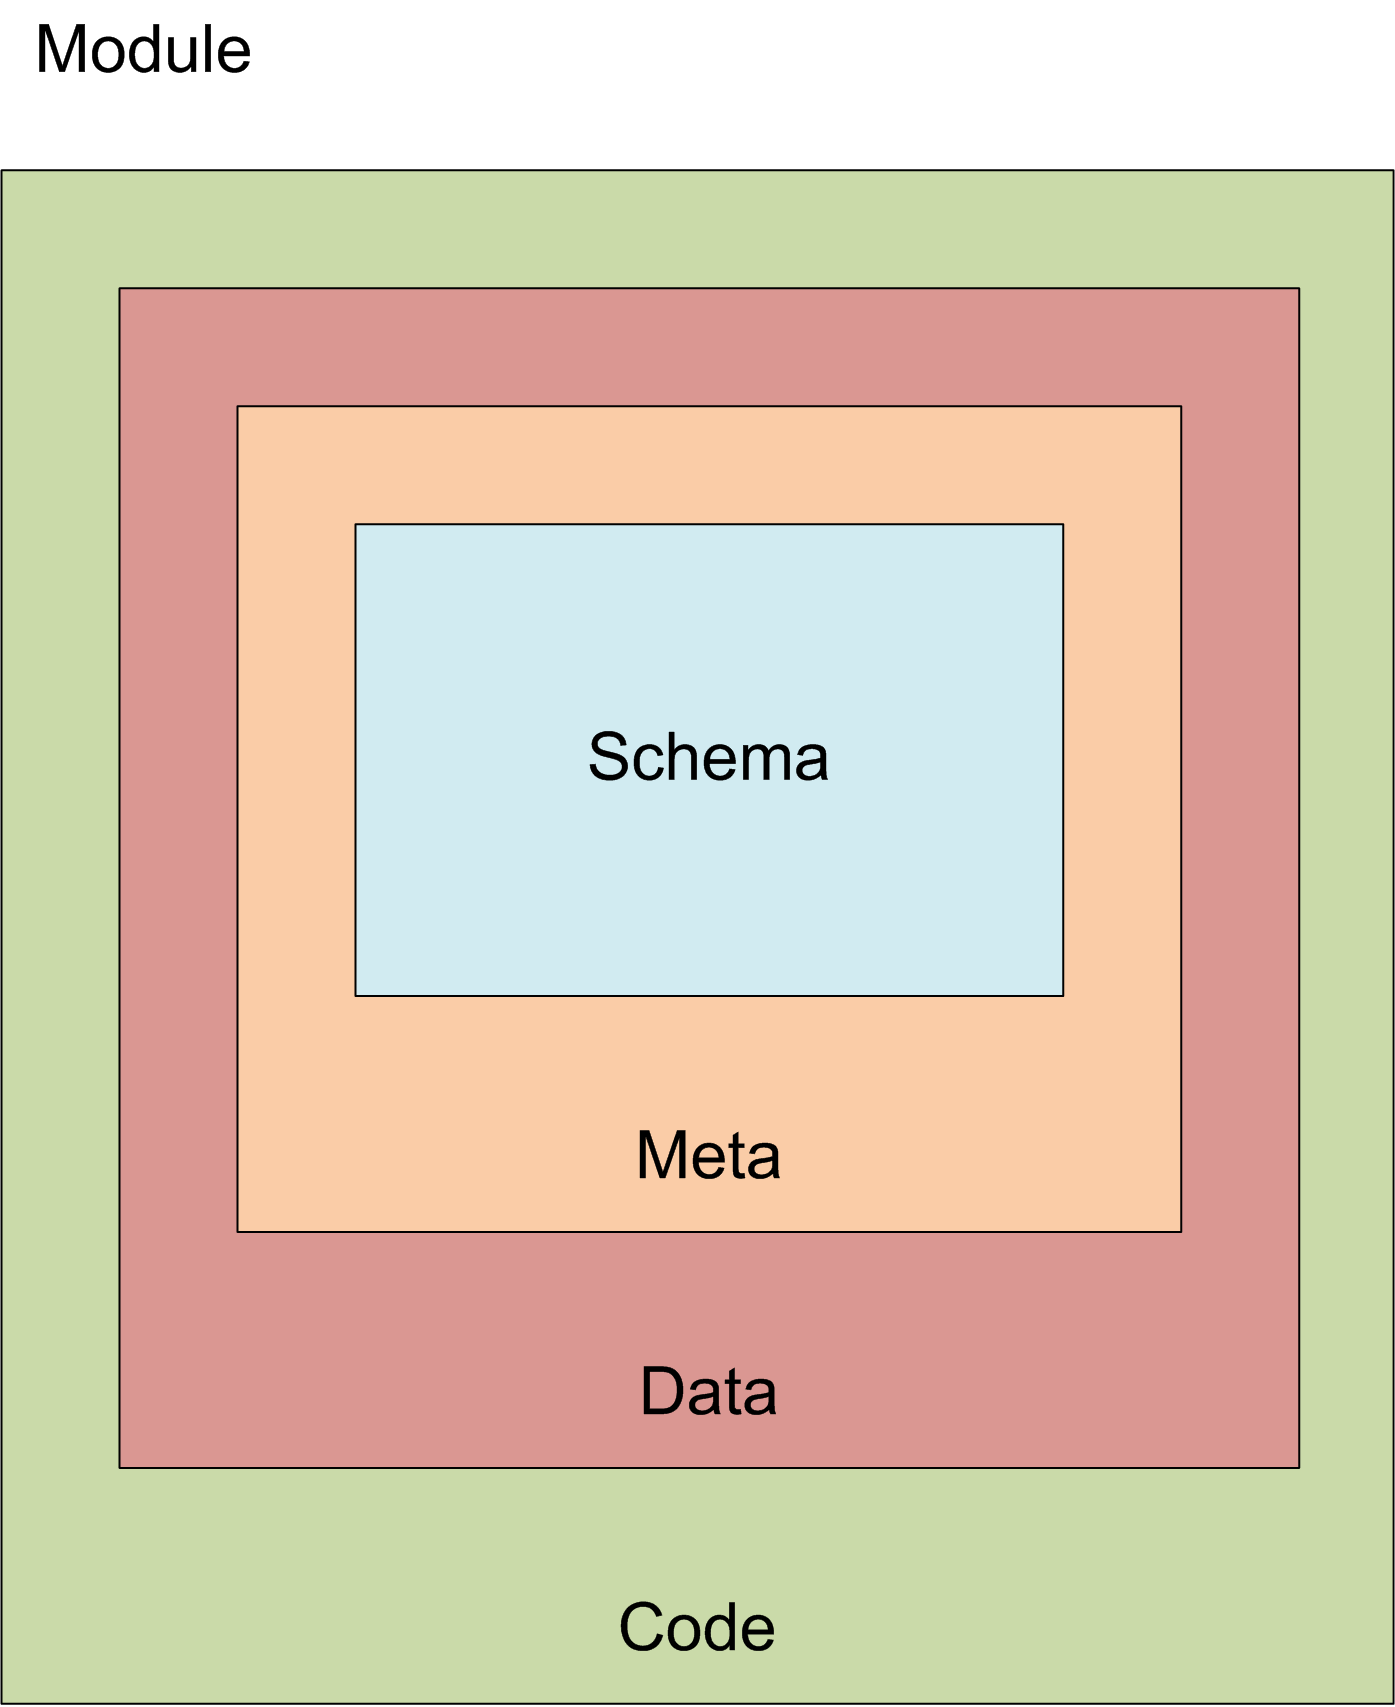
\includegraphics[width=0.6\textwidth]{images/content_of_package.png}
		\caption{Content of a package}
		\label{content_of_package}
	\end{center}
\end{figure}

\subsection{\label{Packaging_Schema}Schema}

Schema contains all information needed by the SchemaManager \ref{} to create or update the database. Schema objects are:

\begin{descriptionBorder}
	\item[DataType] { All object classes and structs except enumerations and interfaces. \emph{To be implemented!} }
	\item[Property] { All properties }
	\item[Relation] { All relations }
	\item[RelationEnd] { All relation ends }
	\item[DefaultPropertyValue] { All known default property values (IntDefaultValue, \ldots) }
	\item[Constraint] { All known constraints (NotNullable, \ldots) }
\end{descriptionBorder}

\par
Schema is a subset of meta data. See \ref{Packaging_Meta}. Currently there is no way to extract schema information without meta information.


\subsection{\label{Packaging_Meta}Meta}

Meta data contains all information needed to describe a Module. That are \emph{ObjectClasses}, \emph{TypeRefs}, \emph{Module} informations, \emph{icons}, \emph{ViewDescriptors} and so on. 
Meta data is a superset of schema data \ref{Packaging_Schema}. These objects are:

\begin{descriptionBorder}
	\item[Module] { The module object }
	\item[ObjectClass\_implements\_Interface\_RelationEntry] { All object class interface relations }
	\item[Method] { All Methods }
	\item[BaseParameter] { All parameter of a method }
	\item[MethodInvocation] { All method invocations }
	\item[PropertyInvocation] { All property invocations (getter/setter) }
	\item[Assembly] { All Assemblies (meta information only, not code) }
	\item[TypeRef] { All type references }
	\item[TypeRef\_hasGenericArguments\_TypeRef\_RelationEntry] { All generic arguments of type references. }
	\item[Icon] { All Icons (descriptor only, no binary data) }
	\item[PresentableModelDescriptor] { All presentable model descriptors }
	\item[ViewDescriptor] { All view descriptors }
	\item[DAVID: ] { please add more GUI objects here. And please do it also in \emph{PackagingHelper.GetMetaObjects(\ldots)} }
\end{descriptionBorder}

Additionally all unknown DefaultPropertyValues and Constraints belongs to meta data.
Meta data can be extracted with the publish command \ref{Packaging_Publish}.

\subsection{\label{Packaging_Data}Data}

A package can also contain additional data. Only object classes that implements \emph{IExportable} will be exported. 
N:M relations between object classes that implements \emph{IExportable} are also exported. 
Currently all objects of a specific module are exported.
Data can be extracted with the export command \ref{Packaging_Export}.

\subsection{\label{Packaging_Code}Code}

Finally a package consists of code in form of assemblies. These assemblies are referenced by \emph{Assembly} objects.

\section{\label{Packaging_Processes}Processes}

\subsection{\label{Packaging_Export}Export}

Exporting is the process of saving objects in XML files. Only object classes that implements \emph{IExportable} will be exported. 
N:M relations between object classes that implements \emph{IExportable} are also exported. 
Currently all objects of a specific module are exported.

Command line for exporting objects:
\begin{CS}
Kistl.Server <configfile.xml> -export <destfile.xml> <namespace> [<namespace> ...]
\end{CS}

The namespace is used to identify a module. \emph{TODO: Work in progress. This is not the best solution!}
\par

This example will export all objects of the project management module:
\begin{CS}
Kistl.Server -export Export.xml Kistl.App.Projekte
\end{CS}

This example will export \emph{all} meta data of \emph{all} modules:
\begin{CS}
Kistl.Server -export Export.xml Kistl.App.Base Kistl.App.GUI
\end{CS}

This example will export the whole database:
\begin{CS}
Kistl.Server -export Export.xml *
\end{CS}

\subsection{\label{Packaging_Import}Import}

Importing is the inverse process of exporting \ref{Packaging_Export}. Objects are imported by the following rules:

\begin{enumerate}
 \item If an imported object already exists in the target database then the object will be overridden
 \item New objects are added
 \item No object is deleted if it's not contained in the package
\end{enumerate}

Command line for importing objects:
\begin{CS}
Kistl.Server <configfile.xml> -import <sourcefile.xml>
\end{CS}

\subsection{\label{Packaging_Publish}Publish}

Publishing is a special case of exporting \ref{Packaging_Export}. Only meta data \ref{Packaging_Meta} of a given module will be exported. 
Additionally only properties of the Kistl.App.Base and Kistl.App.GUI module are published.

Command line for publishing modules:
\begin{CS}
Kistl.Server <configfile.xml> -publish <destfile.xml> <namespace> [<namespace> ...]
\end{CS}

The namespace is used to identify a module. \emph{TODO: Work in progress. This is not the best solution!}
\par

This example will publish the project management module:
\begin{CS}
Kistl.Server -publish Meta.xml Kistl.App.Projekte
\end{CS}

This example will publish all modules:
\begin{CS}
Kistl.Server -publish Meta.xml *
\end{CS}


\subsection{\label{Packaging_Deploy}Deploy}

Deployment is the inverse process of publishing \ref{Packaging_Publish}. It also has different rules (see importing \ref{Packaging_Import}).
These Rules are:

\begin{enumerate}
 \item If an imported object already exists in the target database then the object will be overridden
 \item Only properties of the the Kistl.App.Base and Kistl.App.GUI module are overriden.
 \item New objects are added
 \item Any object that is not contained in the packed will be deleted
\end{enumerate}

Command line for importing objects:
\begin{CS}
Kistl.Server <configfile.xml> -deploy <sourcefile.xml>
\end{CS}

The database schema is not updated. Also no code is generated. This has to be done in an extra step.
\section{\label{Deployment}Deployment}
This section describes the possible deployment strategies. 

\begin{note}
this section is a subject to change
\end{note} 

\subsection{Continuous Integration Server}
The \emph{Continuous Integration Server} does a publish in a directory
structure. This directory structure is transformed by a \emph{fetch} script into the designated
directory structure.

It's not recommended to use the \emph{Continuous Integration Servers} structure
directly. The next section will discuss the fetching process and the designated
directory structure.

\subsection{Fetching and Destination Directory Structure}

The fetching script is responsible for
\begin{itemize}
  \item Creating the directory structure
  \item Fetching all Assemblies and putting them in the right destination
  directory
  \item Copying all app configuration files to the right directories 
\end{itemize} 

The directory structure on the deployment server should look like this:

  	\begin{itemize}
  	  \item AppConfigs
  	  \item { bin
  	  	\begin{itemize}
  	  	  \item Bootstrapper
  	  	  \item { Client
  	  	  	\begin{itemize}
  	  	  	  \item { Client
  	  	  	  	\begin{itemize}
  	  	  	  	  \item App.ZBox
  	  	  	  	  \item Core
  	  	  	  	  \item Core.Generated
  	  	  	  	  \item WPF
  	  	  	  	  \item WinForms
  	  	  	  	 \end{itemize}
  	  	  	  }
  	  	  	  \item { Common
  	  	  	  	\begin{itemize}
  	  	  	  	  \item App.ZBox
  	  	  	  	  \item Core
  	  	  	  	  \item Core.Generated
  	  	  	  	 \end{itemize}
  	  	  	  }
  	  	  	  \item Kistl.Client.WPF.exe
  	  	  	  \item Kistl.Client.WPF.exe.config
  	  	  	  \item Kistl.Client.Forms.exe
  	  	  	  \item Kistl.Client.Forms.exe.config
  	  	  	\end{itemize}  
  	  	  }
  	  	  \item {Server
  	  	  	\begin{itemize}
  	  	  	  \item { Common
  	  	  	  	\begin{itemize}
  	  	  	  	  \item App.ZBox
  	  	  	  	  \item Core
  	  	  	  	  \item Core.Generated
  	  	  	  	 \end{itemize}
  	  	  	  }
  	  	  	  \item { Server
  	  	  	  	\begin{itemize}
  	  	  	  	  \item App.ZBox
  	  	  	  	  \item Core
  	  	  	  	  \item Core.Generated
  	  	  	  	  \item EF
  	  	  	  	  \item EF.Generated
  	  	  	  	  \item NH
  	  	  	  	  \item NH.Generated
  	  	  	  	 \end{itemize}
  	  	  	  }
  	  	  	  \item Kistl.Server.Service.exe
  	  	  	  \item Kistl.Server.Service.exe.config
  	  	  	\end{itemize}  
  		}
  	  	\end{itemize}
  	  }
  	  \item Configs
  	  \item DocumentStore
  	  \item { inetpub
  	  	\begin{itemize} 
  	  	  \item App\_Data
  	  	  \item App\_GlobalResources
  	  	  \item App\_Themes
  	  	  \item bin
  	  	  \item Bootstrapper
  	  	  \item { Common
  	  	  	\begin{itemize}
  	  	  	  \item App.ZBox
  	  	  	  \item Core
  	  	  	  \item Core.Generated
  	  	  	 \end{itemize}
  	  	  }
  	  	  \item { Server
  	  	  	\begin{itemize}
  	  	  	  \item App.ZBox
  	  	  	  \item Core
  	  	  	  \item Core.Generated
  	  	  	  \item EF
  	  	  	  \item EF.Generated
  	  	  	  \item NH
  	  	  	  \item NH.Generated
  	  	  	 \end{itemize}
  	  	  }
  	  	  \end{itemize} 
  	  }
  	  \item logs
  	  \item Packages
  	  \item deploy.ps1
  	  \item fetch.ps1
  	\end{itemize} 

\subsubsection{Root Directory}
\begin{descriptionBorder}
\item[deploy.ps1] The deployment script, responsible for upgrading the servers
database

\item[fetch.ps1] The fetch script, responsible for creating the directory
structure and fetching all assemblies and configuration templates
\end{descriptionBorder}

\subsubsection{AppConfigs}
This directory contains all app configuration files needed by the executing
assemblies. E.g. in the \emph{Kistl.Server.Service.exe.config} all WCF Service
stuff can be configured. In \emph{Kistl.Client.WPF.exe.config} all WCF Proxy
stuff can be configured.

The fetch script will copy those configuration files into the desired
directories, right beside their executalables.

So this is the place where all app specific configuration has to be defined.

Besides WCF stuff, those configuration can be also found in those files:

\begin{itemize}
  \item log4net
  \item WCF
  \item Assembly Bindings
  \item Database provider registration 
\end{itemize} 

\begin{note}
The web.config is not located here, but this may change in the
future
\end{note}

\subsubsection{Configs}
This directory contains all ZBox configuration files. They are located by the
executalable by probing 
\begin{itemize}
  \item the given command line parameter
  \item then the \emph{zenv} environment variable plus executalable name
  \item then each directory up to the \emph{Configs} directory, still with the
  executalable name
  \item at the end by looking for \emph{DefaultConfig.xml} in the configs
  directory
\end{itemize}

\subsubsection{bin}
The bin directory contains all assemblies used by ZBox, divided by theire use
(Bootstrapper, Client or Server). The \emph{Client} and \emph{Server}
directories contains sub directories to split Client/Server and Common parts.
Those directories have for each Application (=ZBox Module) and Modules (not ZBox
Modules!) a individual sub directory.

The naming of Application (=ZBox Module) should be:

\begin{center}
App.\textless ModuleName\textgreater  
\end{center}

\emph{Core} contains all core assemblies like Kistl.API and all other
assemblies that are referenced by default (log4net e.g.).

\emph{Core.Generated} contains all genereated code. Code Generation is done by
the \emph{Continuous Integration Server} so those assemblies will be copied by
the fetch script.

\begin{note}
This is a topic of discussion
\end{note}

\emph{Bootstrapper} contains only one executalable. The Boostrapper itself which
is downloading the whole client application with its configuration from an HTTP
Server via REST.


% \include{ServerAdministration}

% Literature
\begin{thebibliography}{99}

% \bibitem{cpp} Bjarne Stroustrup, The C++ Programming Language,
% Special Edition, 2000, AT\&T Labs, ISBN 0-201-70073-5

% \bibitem{COM} Guy Eddon, Henry Eddon, Inside Distibuted COM,
% 1998, Microsoft Press, ISBN 3-86063-459-3

% \bibitem{ActiveX} Adam Denning, ActiveX Controls Inside Out,
% Second Edition, 1997, Microsoft Press, ISBN 1-57231-350-1

% \bibitem{WIN32API} Richard J. Simon, Win32 Programmierung,
% Band 1, 1996, SAMS, ISBN 3-8272-4502-8

\bibitem{MatViewsWork}Dan Chak, Materialized Views that Really Work,
2008, The PostgreSQL Conference, http://www.pgcon.org/2008/schedule/events/69.en.html

\end{thebibliography}

\listoffigures


\begin{appendix}

% \chapter{Appendix title}

\end{appendix}



\end{document}
